\section{Results and Analysis}
\label{S:t5}
In this section, we discuss the results of applying the proposed framework to the virtual reality data collected. Two data formats are presented and analyzed to test the performance of the algorithms in different conditions. Finally, a game theory-based machine learning interpretability method is applied to a trained model to assess the contribution of contextual variables to the model accuracy.  
\subsection{Implementation Notes}
All data pre-processing and model development are coded in Python programming language, using Keras library and its implementation of TensorFlow with GPU support. After data preparation, an exhaustive grid search is conducted to find the best network configurations. Dropout layers and their rates, number of nodes (neurons) in each hidden layer, batch size, number of hidden LSTM and dense layers, is configured based on a 8-fold cross-validation over 100 epochs, and the best configurations are selected to test on a separate test data set. Models are trained on a Core i7 4GHz CPU and a 16.0 GB memory. 

In total, 3,276 instances of cross were collected using the virtual reality experiments, which is significantly higher than the mid-blocking crossing events detected using all the open-access AV datasets currently available. For distance-based models, each instance of cross is divided into two parts, input to feed the time-series part of the networks, and output to be predicted. Three input proportions ($p$) are tested as the proportion of the length of the road that shapes the input data: 0.3, 0.5, 0.7. The corresponding distance-based data types are named $D\_3,$, $D\_5$ and $D\_7$, respectively. In time-based models on the other hand, each instance of crossing is converted to multiple sequences. Based on model parameters, each $t_1$ second of pedestrian trajectory is used as input to the time-series part of the data, and the following $t_2$ seconds are used as the output to be predicted using the model. Hence, in time-based models, data size is increases significantly compared to distance-based models. Three combinations of sequence duration lengths are tested in this study. In the first generated data of this type, $T\_1\_1$, each 1 second of recorded behaviours of the pedestrian is used to predict the next 1 second. $T\_1\_2$ and $T\_2\_1$ are the two other time-based data types used to train time-based models in this study, with a $t_1$ of 1 and 2 seconds, and a $t_2$ of 2 and 1 seconds, respectively. By using various proportions and formats of the input data, we tried to understand the performance of our proposed algorithm under different scenarios. \cref{tab:datasize} provides the number of samples used for training and testing each of the models, generated from the 3,276 crossing instances. All the models are trained and validated using 80\% of the data, and tested on the remaining 20\%.

To find the best performing model of each type, a grid search of hyperparameters is conducted. Parameters investigated in the search include, batch sizes (32, 64 and 128), dropout rates (0, 0.2 and 0.5), number of nodes (10, 50 and 100), number of hidden LSTM layers(1, 2, and 3) and number of hidden dense layers (1, 2 and 3).     
\begin{table}
\centering
\caption{Number of samples used for training and testing for each data type}
\begin{tabular}{|ll||ll|}
\hline
\textbf{Distance-based} & \textbf{Samples} & \textbf{Time-based} & \textbf{Samples} \\ \hline
$D\_3$                     & 3,261             & $T\_1\_1$               & 58,654            \\ \hline
$D\_5$                     & 3,261             & $T\_1\_2$               & 32,455            \\ \hline
$D\_7$                     & 3,261             & $T\_2\_1$               & 32,455            \\ \hline
\end{tabular}
\label{tab:datasize}
\end{table}

\subsection{Baseline model}
Vanilla LSTM models are used as the base-line model to assess the performance of Aux-LSTM models. The data processing procedure and other configuration setup steps for the base-line models are similar to the Aux-LSTM models. Models are compared based on the error on validation tests, for configuration setups, and test sets, for final model performance assessment. The loss function to be minimized during the training of the models is defined as the Mean Square Error (MSE) of the predicted and ground truth values for the coordinates followed by the pedestrian. Moreover, Root Mean Square Error (RMSE) of the difference between predicted and ground truth coordinates is used as the indicator of the performance of the models.  
\subsection{Distance-based models}
\cref{tab:distmodels} presents the configurations of top distance-based Vanilla and Aux-LSTM models, based on 3 different values of $p$, the proportion of lengths of the road that its corresponding time-series data is used as input to the model. As it can be seen in this table, adding dropout layer has not contributed to better performing models and in all of the 6 top configurations of different models, dropout rate has appeared to be 0. Also, a general trend of a decrease in depth and density of the networks by the increase in the length of input sequence can be observed.  

In addition to model configurations, loss and error over validation and training data is provided in \cref{tab:distmodels}. Comparing Aux-LSTM models with the baseline models, it can be observed that validation errors of all the vanilla models are less than their Aux-LSTM counterpart. The difference in error ranges from around 0.01 meter in D\_3 model with p = 0.3, to around 0.03 meter in D\_7 with an input proportion of 0.7. It can be observed that in general and based on the validation error, including auxiliary information has not helped the model perform better. In addition, with an increase in the length of the time-series input sequence, the contribution of auxiliary information is decreased. The details of the top 5 best performing configurations of distance-based models can be found in \cref{tab:dv3} to \cref{tab:d7}. To asses the performance of the networks more accurately, all the selected trained models are applied to the test dataset. The errors of applying the models on test set over 100 epochs is provided in \cref{tab:Dtest}. According to the table,  performance of all the Aux-LSTM models when applied to the test set is better than the vanilla baseline models. Interestingly, the input proportion with the most accurate models over the validation dataset, i.e. p = 0.7, has the biggest gap between its Aux-LSTM and baseline model. Difference in the performance of the models over validation and test sets can be traced back to the effect of adding auxiliary data to the input sequences and their contribution to the reduction of overfitting in the models. Bigger difference in errors of models with p = 0.7 confirms the idea that having longer sequences of time-series data as input leads to more overfitting to the train data, which is reduced by adding auxiliary information to the input data. In distance-based models with p = 0.3, 0.5 and 0.7, considering auxiliary data in the models has reduced the root mean square error of coordinate predictions by 2\%, 6\% and 17\%, respectively. As stated earlier, the differences between accuracy improvements of the models confirm the extent of overfitting in the models using relatively longer input sequence lengths to predict shorter lengths of output sequence. 

\begin{table}
\centering
\caption{8-fold cross-validation results for top distance-based models}
\label{tab:distmodels}
\scalebox{0.7}{
\begin{tabular}{|lllllllllll|}
\hline
\textbf{p}           & \textbf{Type} & \textbf{\begin{tabular}[c]{@{}l@{}}Dense\\ Layers\end{tabular}} & \textbf{\begin{tabular}[c]{@{}l@{}}LSTM \\ Layers\end{tabular}} & \textbf{Nodes} & \textbf{\begin{tabular}[c]{@{}l@{}}Batch \\ Size\end{tabular}} & \textbf{Dropout} & \textbf{\begin{tabular}[c]{@{}l@{}}Validation \\ Loss \end{tabular}} & \multicolumn{1}{l}{\textbf{\begin{tabular}[c]{@{}l@{}}Validation \\ Error \end{tabular}}} & \textbf{\begin{tabular}[c]{@{}l@{}}Train \\ Loss \end{tabular}} & \textbf{\begin{tabular}[c]{@{}l@{}}Train \\ Error \end{tabular}} \\ \hline
\multirow{2}{*}{0.3} & Aux-LSTM      & 2                                                               & 3                                                               & 100            & 32                                                             & 0                & 0.0219                                                                    & 0.1481                                                                                        & 0.0171                                                               & 0.1306                                                              \\
                     & Vanilla       & NA                                                              & 2                                                               & 100            & 32                                                             & 0                & 0.0180                                                                    & 0.1341                                                                                        & 0.0183                                                               & 0.1351                                                              \\ \hline
\multirow{2}{*}{0.5} & Aux-LSTM      & 2                                                               & 2                                                               & 50             & 128                                                            & 0                & 0.0104                                                                    & 0.1021                                                                                        & 0.0115                                                               & 0.1071                                                              \\
                     & Vanilla       & NA                                                              & 1                                                               & 50             & 128                                                            & 0                & 0.0088                                                                    & 0.0940                                                                                        & 0.0071                                                               & 0.0841                                                              \\ \hline
\multirow{2}{*}{0.7} & Aux-LSTM      & 1                                                               & 3                                                               & 50             & 32                                                             & 0                & 0.0069                                                                    & 0.0830                                                                                        & 0.0059                                                               & 0.0769                                                              \\
                     & Vanilla       & NA                                                              & 1                                                               & 10             & 32                                                             & 0                & 0.0025                                                                    & 0.0500                                                                                        & 0.0030                                                               & 0.0545                                                              \\ \hline
\end{tabular}}
\end{table}

\begin{table}

    \caption{Mean error of test set for selected distance-based models over 100 epochs}
    \centering
    \small\addtolength{\tabcolsep}{-3pt}
    \begin{tabular}{|l|l|l|}
    \hline
       \textbf{ID} & \textbf{Model Type}  & \textbf{Error } \\
       \hline
    
         \textbf{P: 0.3} & Aux-LSTM & 0.3284   \\
           & Vanilla & 0.3307\\
          \hline
         \textbf{P: 0.5}  &  Aux-LSTM & 0.2826  \\
           & Vanilla & 0.3019 \\
         \hline
         \textbf{P: 0.7} & Aux-LSTM & 0.2329  \\
           & Vanilla & 0.2795 \\

    \hline
    \end{tabular}
    \label{tab:Dtest}
\end{table}

\subsection{Time-based models}
Similar steps are followed for time-based models. \cref{tab:timemodels} presents the configurations of top performing time-based models over validation data, as well as their corresponding validation and training error. It is interesting except for number of hidden LSTM layers in T\_2\_1, all the other configurations of the top models appear to be similar to each other. Details of the configurations of top 5 performing time-based models of each data type can be found in \cref{A:valT}, \cref{tab:tv11} to \cref{tab:t21}. 

Unlike distance-based models, all Aux-LSTM time-based models outperform the baseline models over the validation data. Same pattern exists when the models are applied to test set (\cref{tab:Ttest}). Dividing data according to short time intervals of 1 or 2 seconds, has led to shorter sequences, and thus, the models are less prone to overfitting. Hence, the generalizing benefit of auxiliary data is smoothed. However, the performance of the time-based Aux-LSTM models are still better than the baseline models, which is achieved through shorter length of sequences as input data. In general, root mean square errors of coordinate prediction using time-based Aux-LSTM models outperform the baseline models over T\_1\_1, T\_1\_2 and T\_2\_1 data types by 7\%, 12\% and 12\% respectively. Compared to distance-based models, the gap between accuracy improvements of different time-based data types is smaller, which can be traced to the smaller differences in input and output sequence lengths in time-based data.

\begin{table}
\centering
\caption{8-fold cross-validation results for top time-based models}
\label{tab:timemodels}
\scalebox{0.68}{
\begin{tabular}{|llllllllllll|}
\hline
\textbf{$t_1$ }    & \textbf{$t_2$ }    & \textbf{Type} & \textbf{\begin{tabular}[c]{@{}l@{}}Dense\\ Layers\end{tabular}} & \textbf{\begin{tabular}[c]{@{}l@{}}LSTM \\ Layers\end{tabular}} & \textbf{Nodes} & \textbf{\begin{tabular}[c]{@{}l@{}}Batch \\ Size\end{tabular}} & \textbf{Dropout} & \textbf{\begin{tabular}[c]{@{}l@{}}Validation \\ Loss \end{tabular}} & \multicolumn{1}{l}{\textbf{\begin{tabular}[c]{@{}l@{}}Validation \\ Error \end{tabular}}} & \textbf{\begin{tabular}[c]{@{}l@{}}Train \\ Loss \end{tabular}} & \textbf{\begin{tabular}[c]{@{}l@{}}Train \\ Error \end{tabular}} \\ \hline
\multirow{2}{*}{1} & \multirow{2}{*}{1} & Aux-LSTM      & 3                                                               & 2                                                               & 100            & 32                                                             & 0                & 0.0181                                                                    & 0.1344                                                                                        & 0.0085                                                               & 0.0922                                                              \\
                   &                    & Vanilla       & NA                                                              & 2                                                               & 100            & 32                                                             & 0                & 0.0312                                                                    & 0.1767                                                                                        & 0.0170                                                               & 0.1304                                                              \\ \hline
\multirow{2}{*}{1} & \multirow{2}{*}{2} & Aux-LSTM      & 3                                                               & 2                                                               & 100            & 32                                                             & 0                & 0.0305                                                                    & 0.1748                                                                                        & 0.0139                                                               & 0.1178                                                              \\
                   &                    & Vanilla       & NA                                                              & 3                                                               & 100            & 32                                                             & 0                & 0.0781                                                                    & 0.2795                                                                                        & 0.0322                                                               & 0.1795                                                              \\ \hline
\multirow{2}{*}{2} & \multirow{2}{*}{1} & Aux-LSTM      & 3                                                               & 3                                                               & 100            & 32                                                             & 0                & 0.0068                                                                    & 0.0827                                                                                        & 0.0049                                                               & 0.0700                                                              \\
                   &                    & Vanilla       & NA                                                              & 2                                                               & 100            & 32                                                             & 0                & 0.0097                                                                    & 0.0983                                                                                        & 0.0053                                                               & 0.0726                                                              \\ \hline
\end{tabular}}
\end{table}
\begin{table}

    \caption{Mean error of test set for selected time-based models over 100 epochs}
    \centering
    \small\addtolength{\tabcolsep}{-3pt}
    \begin{tabular}{|l|l|l|}
    \hline
       \textbf{ID} & \textbf{Model Type}  & \textbf{Test Error } \\
       \hline
    
         \textbf{$t_1$: 1, $t_2$: 1}  & Aux-LSTM &  0.2606   \\
         \textbf{}  & Vanilla & 0.2801\\
         \hline
         \textbf{$t_1$: 1, $t_2$: 2} & Aux-LSTM & 0.3642     \\
          & Vanilla & 0.4122 \\
         \hline
         \textbf{$t_1$: 2, $t_2$: 1}  & Aux-LSTM & 0.2707\\
            & Vanilla &  0.3083 \\
    \hline
    \end{tabular}
    \label{tab:Ttest}
\end{table}

\subsection{Interpretation of the results}
A major criticism of neural networks, and one of the main barriers toward even more prevalence of them specially in practical applications is the difficulties involved in their interpretability, and their \textit{black box} nature. As this study suggests Virtual Reality data as a tool to complement AV datasets, providing insights on the contributing factors to the error in trajectory prediction of pedestrians can be beneficial to future AV data collections, as well as current AV data analysis. In this section, we implement SHAP, a post-hoc game theory-based interpretation method, to understand the effect of variables on the prediction error.

Shapley value is a method in rooted in game theory to allocate the payoff of a job done in coalition, to the involved contributors. The same concepts can be applied in determining the contribution of each variable to the model output. Shapley value of each variable $i$ is calculated as follows~\cite{lipovetsky2001analysis}:

\begin{linenomath}
\begin{equation}
\label{eq:shapley}
\Phi_i = \sum_{S \in F \setminus \{i\}} \frac{|S|! (|F| - |S| -1)!}{|F|!} \left(
g_{S\cup\{i\}}(Z_{S\cup\{i\}}) - g_S(Z_S) \right)
\end{equation}
\end{linenomath}
In \cref{eq:shapley}, $S$ is a subset of all variables, $F$, $g_{S\cup\{i\}}$ is the model trained using a subset with variable $\{i\}$ present, and $g_S$ is the model trained without the variable $i$. Lundberg~\textit{et al.}~\cite{lundberg2017unified} applied the concept of Shapley values to model interpretation and proposed to estimate the importance of a variable in an instance based on the corresponding Shapley values.

\cref{fig:Tshap} plots the summary of the SHAP values applied to the Aux-LSTM model trained on T\_1\_1 data. The effect of variables on the error in predicting trajectory of pedestrians is provided in this plot. Having a positive SHAP values for a variable in an instance means higher error due to presence of that factor. The most contributing variable to the error is snow. According to the figure, in all the instances with snowy weather in the scenario the error in prediction is increased. Similar trend holds true in night scenarios, with the majority of instances in night scenarios leading to an increase in error prediction. With the affected sight distance in night and snowy environments, participants were expected to follow more erratic trajectories. High impact of weather conditions in the VR environment shows the importance of environmental diversity in AV datasets. Regarding the variable related to speed limit, it can be observed in the plot that in lower speeds the models are able to predict the trajectory more accurately. It can be concluded that in our experiment, participants were behaving more predictably when confronting slower traffics. The same behaviour can be seen in scenarios with lower vehicle flow rates. In most instances with a low flowe rate (530 veh/hr), the SHAP value of the corresponding arrival rate variable is negative, meaning the positive impact of this variable on achieving higher accuracies in trajectory prediction. Assuming more stress levels of participants when confronting faster or more congested traffics, more uncertain and unpredictable trajectories in these conditions can be explained. Another significantly contributing variable seems to be the road type. In the scenarios with a two-way road and median, the prediction has higher errors, showing a more unpredictable trajectory of pedestrians when facing vehicles in two directions. Finally, lane width variables do not seem to have a consistent impact on the instances, with SHAP values in different instances spreading on the both sides of the spectrum. In general, contextual information on traffic characteristics, road geometry, and weather conditions appear to have the greatest impact on the error of the model. Based on these observations, we recommend taking into account such variables during the data collection and modeling behaviour of pedestrians when interacting with AVs. All the variables included in the model were set in a way that a typical AV can capture or calculate based on the information obtained by its camera, LIDAR, or other sensors available to them.

\begin{figure}
    \centering
    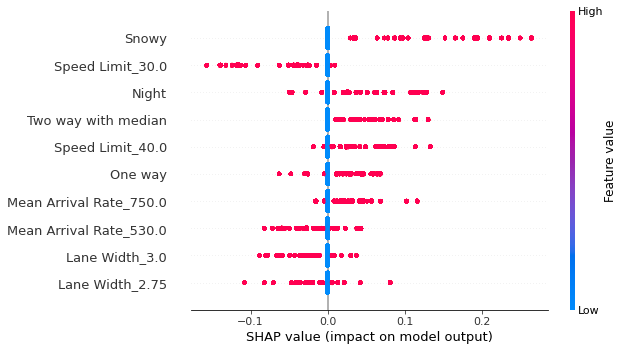
\includegraphics[scale=0.6]{chapter_6/figures/shaptraj2.png}
    \caption{Plot summary of the effects of auxiliary variables on error}
    \label{fig:Tshap}
\end{figure}

